\documentclass{article}
\usepackage[utf8]{inputenc}
\usepackage{graphicx}

\title{Intelligens fejlesztőeszkozok}
\author{Burian Sándor}
\date{Szeptember 2022}

\begin{document}

\maketitle

\section{1. beadandó}

Azért Textmaker és MIKTeXet használok, mert ezt ajánlották internetes fórumokon, és blogokban mint második legjobb latex editor windowsra az Overleaf után.

Alább látható kép a sinus plotról és a futó Julia kódról valamint a LaTeX szerkesztőről.
\begin{figure}
    \centering
	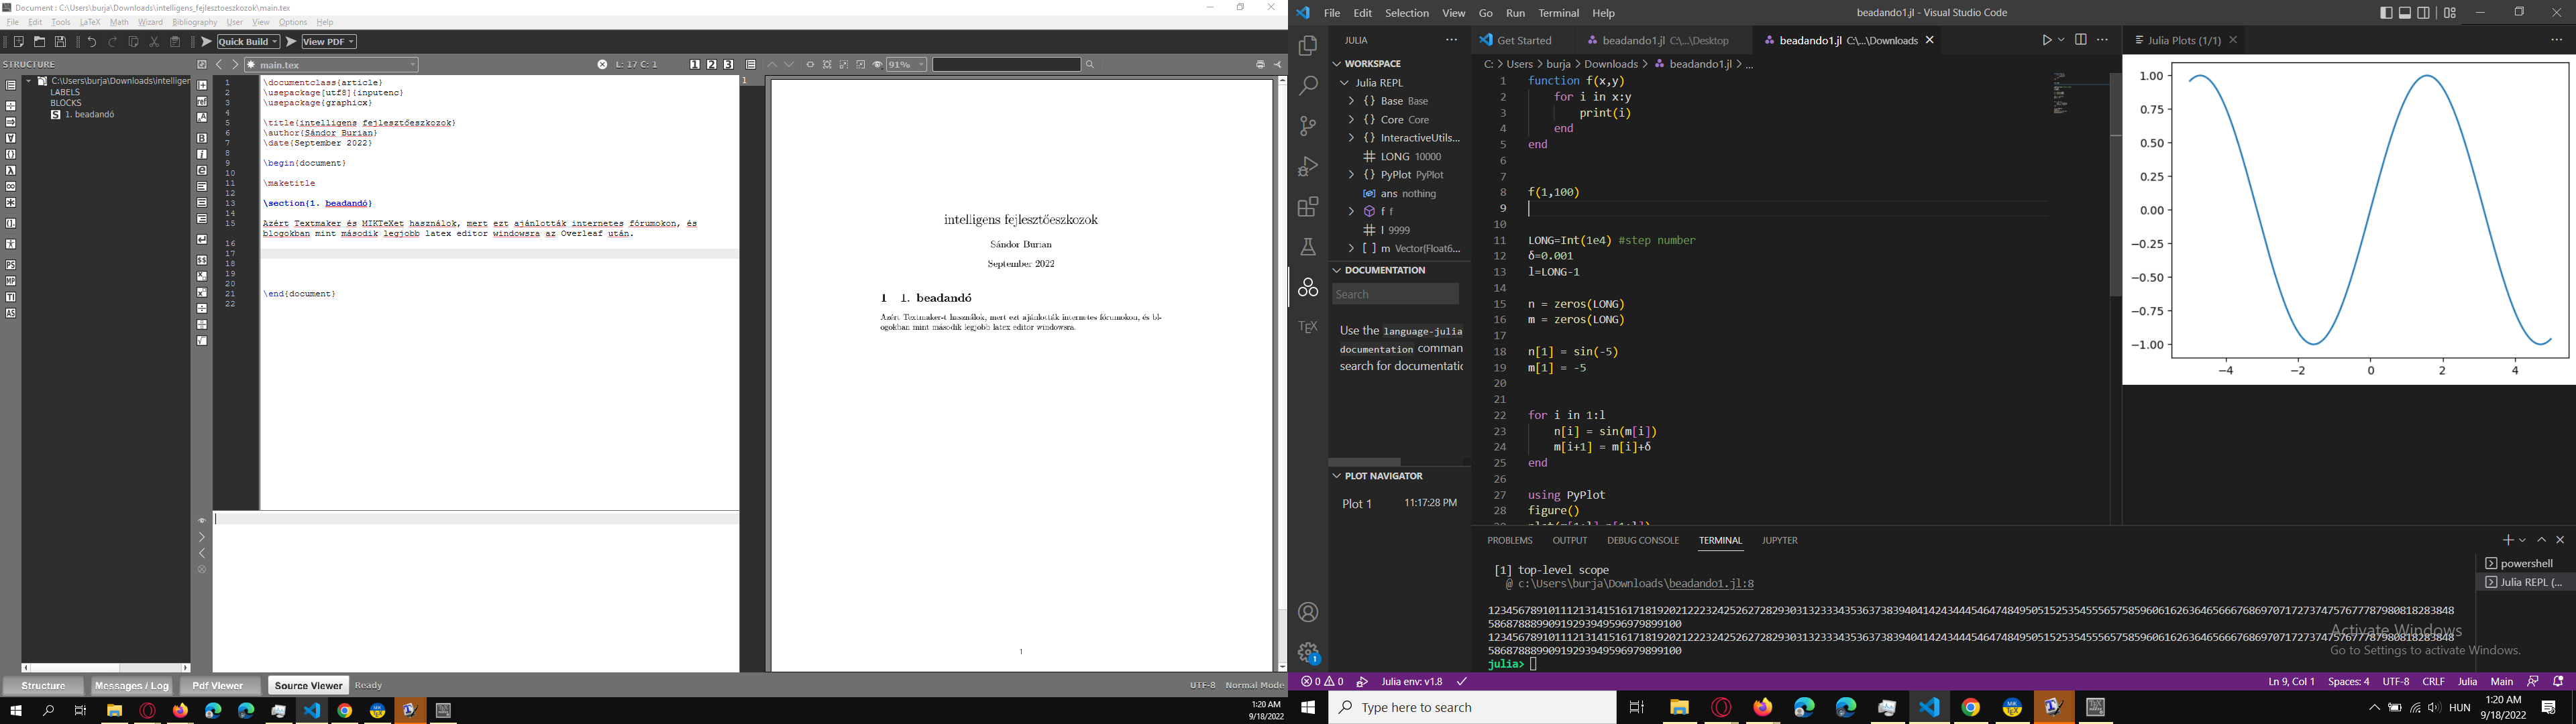
\includegraphics[width=15cm]{kepernyokep_ujra.png} 
    \caption{képernyőkép Texmakerről és futó Julia kódról}
    \label{fig:képernyőkép Texmakerről és futó Julia kódról}
\end{figure}



\end{document}
